\tikzstyle{startstop} = [rectangle, rounded corners, minimum width=3cm, minimum height=1cm,text centered, draw=black, fill=red!30]
\tikzstyle{io} = [trapezium, trapezium left angle=70, trapezium right angle=110, minimum width=3cm, minimum height=1cm, text centered, draw=black, fill=blue!30]
\tikzstyle{process} = [rectangle, minimum width=3cm, minimum height=1cm, text centered, draw=black, fill=orange!30]
\tikzstyle{decision} = [diamond, minimum width=3cm, minimum height=1cm, text centered, draw=black, fill=green!30]
\usetikzlibrary{shapes.geometric}
\tikzstyle{database} = [cylinder, minimum width=3cm, minimum height=1cm, text centered, draw=black, fill=yellow!30, shape border rotate=90, aspect=0.25]

\chapter{Atomic Pair Distribution Function: \\Theory and Computation}
\section{Theory}
To properly understand the PDF and its limitations we need to derive its mathematics.
The following derivation has been performed numerous times but most recently and completely by Farrow and Billinge, it is reproduced here for clarity and completeness.
\subsection{Derivation}
\subsection{Analytical Gradients}
Many optimization algorithms and simulations methodologies, including HMC, require not only the potential energy of a given configuration but also the forces acting on that configuration.
These forces are described by the gradient of potential energy of the system which in turn requires the gradient of the PDF.
As previously shown the PDF is the Fourier Transform of the Debye equation.
Since the Fourier Transform is expressed as an integral we can exchange the order of the gradient and the integral, allowing us to calculate the analytical gradient of the Debye equation and FFT the resulting function.
The Debye equation, with a Debye-Waller vibrational correction is
\begin{equation}
F(Q) = \frac{1}{N \langle f \rangle^{2}} \sum_{j\neq i} f_i^{*}(Q)f_j(Q) \exp(-\frac{1}{2}\sigma_{ij}^{2}Q^{2}) \frac{\sin(Qr_{ij})}{r_{ij}}
\end{equation}
where
\begin{eqnarray}
  \sigma_{ij}^{2} = (\vec{u}_{ij} * \hat{d}_{ij})^{2}\\
  \vec{u}_{ij} = \vec{u}_{i} - \vec{u}_{j}\\
  \hat{d}_{ij} = \frac{\vec{d}_{ij}}{r_{ij}}\\
  r_{ij} = ||\vec{d}_{ij}|| \\
  \vec{d}_{ij} =
  \begin{bmatrix}
    q_{ix} - q_{jx}\\
    q_{iy} - q_{jy} \\
    q_{iz} - q_{jz}
  \end{bmatrix}
\end{eqnarray}
where $Q$ is the scatter vector, $f_i$ is atomic scattering factor of the $i$th atom, and $r_{ij}$ is the distance between atoms $i$ and $j$ and has $q$ dependence.
For simplicities sake we will break up $F(Q)$ so that
\begin{equation}
F(Q) = \alpha \sum_{j\neq i} \beta_{ij} \uptau_{ij} \Omega_{ij}
\end{equation}
where
\begin{eqnarray}
  \alpha = \frac{1}{N \langle f \rangle^{2}} \\
  \beta_{ij} = f_i^{*}(Q)f_j(Q)\\
  \uptau_{ij} = \exp(-\frac{1}{2}\sigma_{ij}^{2}Q^{2})\\
  \Omega_{ij} = \frac{\sin(Qr_{ij})}{r_{ij}}
\end{eqnarray}

\noindent The derivatives are as follows:
\begin{equation}
\frac{\partial}{\partial q_{i,w}} F{ (Q )} = \alpha \sum_{j} \beta_{ij} (\frac{\partial \uptau_{ij}}{\partial q_{i,w}}  \Omega_{ij} + \uptau_{ij} \frac{\partial \Omega_{ij}}{\partial q_{i,w}})
\end{equation}
where
\begin{eqnarray}
  \frac{\partial \Omega_{ij}}{\partial q_{i,w}}  = \frac{Q\cos(Qr_{ij}) - \Omega_{ij}}{r_{ij}^{2}} (q_{i,w}-q_{j,w})\\
  \frac{\partial \uptau_{ij}}{\partial q_{i,w}} = \frac{\sigma_{ij}Q^{2} \uptau_{ij}}{r_{ij}^{3}}   ((q_{i,w} - q_{j,w}) \sigma_{ij}- ( u_{i,w} - u_{j,w})r_{ij}^{2})
\end{eqnarray}

Since $\vec{u}_{ij}$ is a variable as well, we need the derivative with respect to it as well.
Thus
\begin{equation}
\frac{\partial}{\partial u_{i,w}} F{ (Q )} = \alpha \sum_{j} \beta_{ij} \frac{\partial \uptau_{ij}}{\partial u_{i,w}}  \Omega_{ij}
\end{equation}

\begin{eqnarray}
\frac{\partial \uptau_{ij}}{\partial u_{i,w}} =
- \frac{\sigma_{ij}Q^{2} \uptau_{ij}}{r_{ij}}  (q_{i,w} - q_{j,w})
\end{eqnarray}
\subsubsection{Without ADPs}
Without ADPs the equations simplify down to
\begin{equation}
F(Q) = \frac{1}{N \langle f \rangle^{2}} \sum_{j\neq} f_i^{*}(Q)f_j(Q) \frac{\sin(Qr_{ij})}{r_{ij}}
\end{equation}
and
 \begin{equation}
\frac{\partial}{\partial q_{i,w}} F{ (Q )} = \alpha \sum_{j} \beta_{ij} \frac{\partial \Omega_{ij}}{\partial q_{i,w}}
\end{equation}
use of these equations, when ADPs are not appropriate (like at cyrogenic temperatures), greatly speeds up the computaiton.

\section{Computation}
Simply deriving the equations for the PDF is not enough.
The many body nature of the PDF equation make analytical solution of the structure from the PDF impossible.
Thus, the PDF must be computed from a structural candidates and compared against experimental results to evaluate the relability of the model.

\subsection{HPC and GPUs}
To properly solve the structure of materials the PDF will need to be computed many times and checked against experimental results.
This requires computation of the PDF, potentialy over many atoms.
Calculating these PDFs requires a fast, highly parallized, computational framework.
\subsubsection{GPUs and Parallelization}
Computing the PDF is an embarrassingly parallel problem.
The basic procedure is to calculate the reduced structure factor $F(Q)$ for each atom pair and momentum transfer vector, sum over all the atom pairs, and Fourier transform the structure to the PDF.
The first part of this procedure is perfectly parallizable, as each atom pair is seperate from the others.
The summation over all the atomic reduced structure factors can be parallelized via distributed summing.
Lastly the FFT can be parallelized using existing parellel FFT algorithms.

GPUs are particularly well suted to the task of computing PDFs.
GPU chip architecture is designed to perform many task simultaniously by having potentially thousands of cores.

\subsubsection{Map from ij space to k space}
The above equations, although formally correct, are very ineffiecent. $F(Q)$ and its gradient are indexed over all the atoms twice, however there are symmetries that allow us to only compute over the atom pairs esentially mapping from an $n$x$n$ space, $ij$ space, to a $\frac{n(n-1)}{2}$ space, $k$ space.
For $F(Q)$ we apply the following mapping
\begin{figure}[!ht]
\begin{center}
\begin{tikzpicture}
    \node (E) at (0,0) {$E$};
    \node[right=of E] (F) {$E'$};
    \node[right=of F] (Z) {$Z$};
    \node[below=of F] (N) {$B'$};
    \node[below=of E] (M) {$B$};
    \draw[->] (E)--(F) node [midway,above] {$\psi$};
    \draw[->] (F)--(Z) node [midway,above] {$\Sigma$};
    \draw[->] (M)--(N) node [midway,below] {$\psi'$};
    \draw[->] (E)--(M) node [midway,left] {$\phi$};
    \draw[->] (N)--(Z) node [midway,left] {$\Sigma'$};
\end{tikzpicture}
\end{center}
\end{figure}
where $E$ denotes the atomic coordinates in $ij$ space, $E'$ denotes $F(Q)$ before the summation in $ij$ space, $B$ denotes the atomic pairs in $k$ space, $B'$ denotes $F(Q)$ in $k$ space, and $Z$ denotes the final summed $F(Q)$.  For the operators, $\phi$ denotes the mapping from $ij$ space to $k$ space $k = j + i * \frac{i - 1}{2}$, $\psi$ and $\psi'$ denote the $F(Q)$ operation in $ij$ and $k$ space, respectivly. $\Sigma$ denotes the sum over all the atoms.  

To properly define $\Sigma'$ we must establish whether $F(Q)$ is an even function.  
We can accomplish this by examining each of the portions of $F(Q)$, $\alpha, \beta ,\uptau, \Omega$.
$\Omega$ is even, since $r_{ij}$ is the interatomic distance, which is the same despite a flip of indicies, $Q$ does not depend on the atomic indicies, and since $Qr_{ij}$ is even so is $\sin{Qr_{ij}}$.  Thus, $\Omega$ is even.  Providing similar analysis to $\uptau$ we can see that while $\vec{u}_{ij}$ is odd, so is the unit displacement vector between the two atoms, thus the two odds cancel out.
Intuitivly this makes sense, since the $F(Q)$ equation is fundamentally interested in the interatomic distances which is even.  Thus, switching atom indicies does not change $F(Q)$.
Due to the even nature of the $F(Q)$ operator the $\Sigma'$ operator sums over all the atom pairs, and multiplies by two to reflect the double counting of the $\Sigma$ operator.

For the gradient a similar mapping is used:
\begin{figure}[h!]
\begin{center}
  \begin{tikzpicture}
    \node (E) at (0,0) {$E$};
    \node[right=of E] (F) {$E'$};
    \node[right=of F] (Z) {$Z$};
    \node[below=of F] (N) {$B'$};
    \node[below=of E] (M) {$B$};
    \draw[->] (E)--(F) node [midway,above] {$\psi$};
    \draw[->] (F)--(Z) node [midway,above] {$\Sigma$};
    \draw[->] (M)--(N) node [midway,below] {$\psi'$};
    \draw[->] (E)--(M) node [midway,left] {$\phi$};
    \draw[->] (N)--(Z) node [midway,left] {$\tilde{\phi}\Sigma$};
\end{tikzpicture}
\end{center}
\end{figure}

In this mapping, however, we use the $\tilde{\phi}\Sigma$ operator.  This operator simultaniously performs a reverse mapping from $k$ to $ij$ space, and a summation with the correct symmetry.  In this case the $\psi$ and $\psi'$ operators, which denote the $\grad{F(Q)}$ operator in $ij$ and $k$ space, are antisymmetric.  Intuitivly this makes sense as an extension of Newton's Second Law, since each particle's interation is felt oppositely by its partner.
\subsubsection{Periodic Boundary Conditions}
Periodic boundary conditions can be helpful when simulating extended solids or large nanoparticles. In this case all the non-crystallinity is contained within the simulation box and the box is repeated to create the longer distance peaks observed in the PDF. To perform this we can break up the Debye equation into two main parts, the part that describes the interatomic distances within the simulation box and those between boxes. Neglecting the thermal motion portion:
\begin{equation}
  F(Q) = \frac{1}{N \langle f \rangle^{2}}(\sum_{j\neq i} f_i^{*}(Q)f_j(Q) \frac{\sin(Qr_{ij})}{r_{ij}} + \sum_{i,j} f_i^{*}(Q)f_j(Q) \frac{\sin(QR_{ij})}{R_{ij}})
\end{equation}
where 
\begin{eqnarray}
  R = |\vec{r} + \vec{u}|\\
  \vec{u} = \gamma_1*\vec{a} + \gamma_2*\vec{b} + \gamma_3*\vec{c}
\end{eqnarray}
\section{Experiment}
PDF experiments are generally performed at synchrotron light sources, as only these sources can provide the need flux, energy, and high momentum transfer vectors needed to obtain relyable PDFs.

\section{Data Processing Workflow}
Processing the raw pixel intensities to the PDF is very important as we are extracting most of our interesting information out of very high $Q$ data.
This data relies on good statistics and sound background subtraction.
Talk about papers from Billinge Group with thin film PDF and dilute NP solutions.
Diagram of the overall data processing workflow.
Discuss the NSLS-II data stack.
\begin{figure}
\centering
\begin{tikzpicture}[thick,scale=0.6, every node/.style={scale=0.6}]
    \node (img) [startstop] at (0,0) {Image Data};
    \node [database, right=of img] (fs)  {FileStore};
    \node[startstop, below=of img] (imeta) {Image Metadata};
    \node[startstop, below=of imeta] (emeta) {Environmental Metadata};
    \node[startstop, below=of emeta] (bmeta) {Beamline Metadata};
    \node[startstop, below=of bmeta] (smeta) {Sample Metadata};
    \node[database, right=of emeta] (mds) {MetadataStore};
    \node[process, right=of mds] (db) {DataBroker};
%     \node[io, right=of db] (lfg) {Load Data};
%     \node[io, below=of lfg] (lbg) {Load Background};
%     \node[process, right=of lfg] (maskfg) {Mask Data};
%     \node[process, right=of lbg] (maskbg) {Mask Background};
%     \node[process, right=of maskfg] (ifg) {Azimuthally Integrate Data};
%     \node[process, right=of maskbg] (ibg) {Azimuthally Integrate Background};
%     \node[process, right=of ifg] (bgsubs) {Subtract Background};

%     \draw[->] (img) -- ++(0,1) -- ++($(fs)+(0,1)$)node[] -- (fs);
%     \draw[->] (F)--(Z) node [midway,above] {$\Sigma$};
%     \draw[->] (M)--(N) node [midway,below] {$\psi'$};
%     \draw[->] (E)--(M) node [midway,left] {$\phi$};
%     \draw[->] (N)--(Z) node [midway,left] {$\tilde{\phi}\Sigma$};
\end{tikzpicture}
\caption{Database Loading Workflow. Data is loaded from various sources, including images and text files, into the FileStore and MetadataStore databases. Data is then retrieved from the databases using the databroker.}
\end{figure}
\subsection{MetadataStore Side Loading}
Design of sidewinder-spec for loading the data into metadatastore.
Most of the design considerations went into the loaders, which are different for each experiment.
\subsection{Automated Image Azimuthal Integration}
Mux data as needed. 
Use pyFAI to get the radial distance array.
Note that to properly mask and integrate the system we need to compute the bin edges for the pixels.
The bin edges change as a function of $Q$, as the angle subtended by a pixel shrinks essentially giving high $Q$ pixels more resolution.

\subsection{Detector $Q$ resolution} \label{subsec:qres}
\begin{figure}[!ht]
  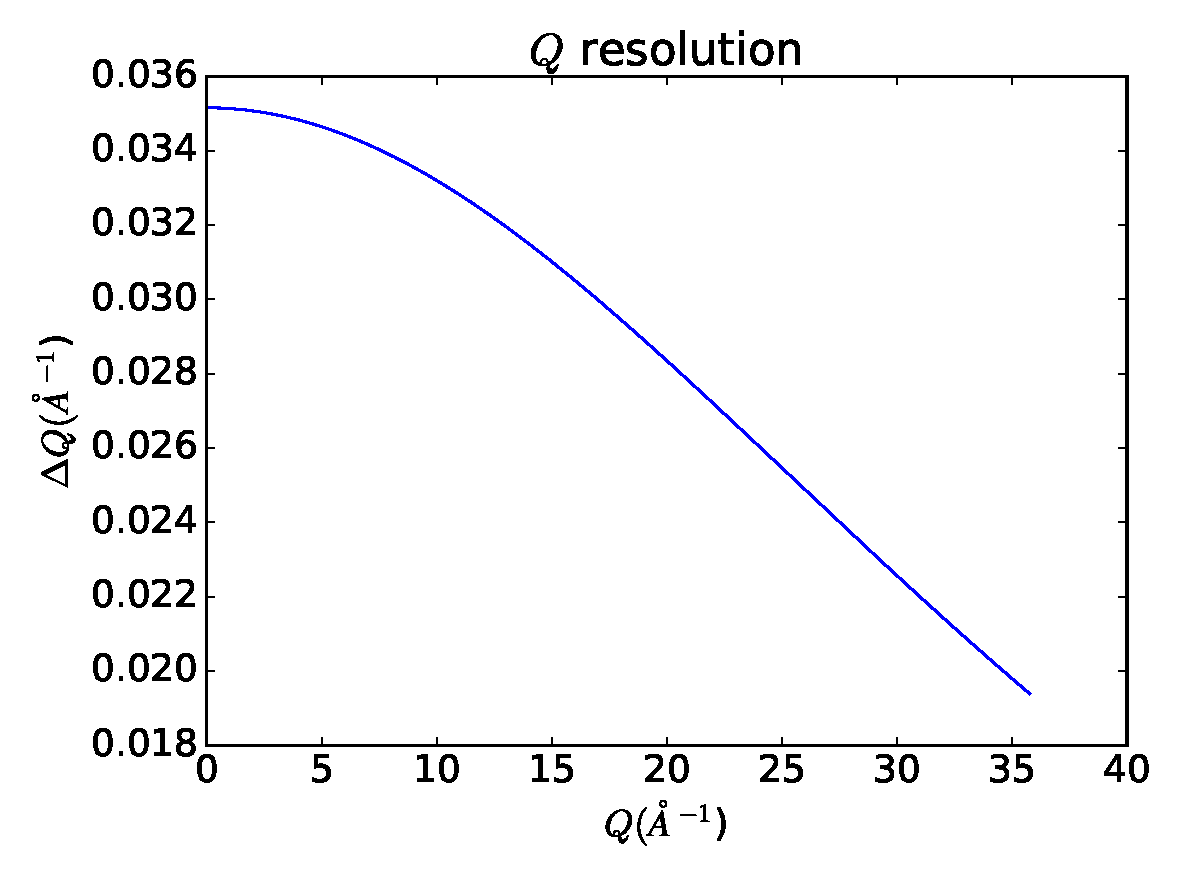
\includegraphics[width=\textwidth]{res}
\caption{$Q$ resolution as a function of $Q$.}
\end{figure}

\subsection{Automated Mask Generation}
\subsubsection{Introduction}
Detector masking is an important part of any x-ray scattering workflow as dead/hot pixels, streak errors, and beamstop associated features can be averaged into the data changing the signal and its statistical significance.
While some features, like the beamstop holder, can be easily observed and masked by hand other are much more difficult to observe even on large computer monitors.
Additionally, while dead/hot pixels and streaks are usually static the hot pixels associated with textured or single crystal scattering or cosmic rays are not.
Thus, coming up with an automated method for finding such erroneous pixels is important, especially as high flux diffraction beamlines can generate data very quickly.

While this problem can be quite complex in the most general case, we can use the annular symmetry of the powder scattering pattern to our advantage, by comparing a pixel against pixels in the same ring.
Since non-textured powder scattering should produce the same pixel intensity for a given ring we can mask any pixels which are $\alpha$ standard deviations away from the mean.
This method relies on the aforementioned pixel binning algorithm, as using miss sized bins will cause some pixels which should be in separate rings to be put together, and others which should be in the same ring to be separated.
In that case the masking algorithm will overestimate the number of pixels to be masked due to the additional statistical variation in the sample.

\subsubsection{Algorithm Design}
The masking algorithm procedure takes in the image and a description of the pixel positions in either distance from the point of incidence or in $Q$.
The image is then integrated twice, producing both the mean $I(Q)$ and the standard deviation of each $I(Q)$ ring.
The mask is created by comparing the pixel values against each ring's standard deviation and theshold $\alpha$.
Note that the theshold can be a funciton of distance from the point of incidence or $Q$.

\subsubsection{Test Cases}
To study the effectiveness of the masking we ran the algorithm against both simulated experimental data.
In the case of the simulated data four systems were created:
1) dead/hot pixels with varying numbers of defective pixels,
2) beamstop holder vith varying beamstop holder transmittance,
3) rotated beamstop holder vith varying beamstop holder transmittance,
and 4) beamstop holder with dead/hot pixels.
The base scattering was produced by
\begin{equation}
I = 100\cos(50r)^{2} + 150
\end{equation}
where $r$ is a pixel's distance from the beam point of incidence.
The positions of the dead/hot pixels were chosen at random as was the dead or hot nature of the defect. Dead pixels had values from 0 to 10, while hot pixels had values from 200 to 255.
The beamstop was positioned at the vertical center of the detector with an initial width of 60 pixels and final width of 120 pixels.
The hight of the beamstop was 1024 pixels.
The beamstop was calculated to attenuate the x-ray scattering signal at various transmittance, as various beamstop holder materials have different transmittance.
Two version of the masking algorithm were run for each test case, one using the standard even bin sizes for the integration step, and one where the bin sizes are tuned to the pixel $Q$ resolution as discussed in \ref{subsec:qres}.

\subsubsection{Results and Discussion}

\foreach \n in {100, 300, 500, 1000}{
\begin{figure}
  \centering
  \foreach \m in {masked}{
    \subfloat[]{\includegraphics[width=.5\textwidth]{bad_bin_dead_pixel_\m_\n}}
    \subfloat[]{\includegraphics[width=.5\textwidth]{dead_pixel_\m_\n}}
    }
\caption{Generated dead/hot pixel masks for a detector with $\n$ bad pixels. a) the poorly binned mask and b) the properly binned mask}
  \label{fig:dead_pixel_\n}
\end{figure}
}

\foreach \n in {10, 30, 50, 90}{
\begin{figure}
  \foreach \m in {raw, masked, missed}{
    \subfloat[]{\includegraphics[width=.3\textwidth]{\m_\n}}
    }
  \caption{Generated beamstop holder masks for a beamstop holder with $\n\%$ transmittance. a) the raw image, b) the masked image, c) and the missed pixels}
  \label{fig:bs_\n}
\end{figure}
}

\begin{figure}
        \foreach \m in {raw, masked, missed}{
        \subfloat[]{\includegraphics[width=.3\textwidth]{rotate_\m_50}
        }}
    \caption{Generated beamstop holder masks which is rotated away from verticle}
    \label{fig:rot_bs}
\end{figure}

\begin{figure}
    \includegraphics[width=\textwidth]{single_xtal_masked}
    \caption{Experimental data, with single crystal peaks}
    \label{fig:}
\end{figure}
%MAYBE ALSO ALSO NEED TO SHOW THE EFFECT OF CHANGING ALPHA FOR THE MASKING

ALSO ALSO ALSO SHOW SOME MASKS OF REAL DATA, INCLUDING DATA WITH SINGLE CRYSTAL/TEXTURE

Figures \ref{fig:dead_pixel_100}-\ref{fig:bs_90} show the results of the masking algorithm on simulated images.
The dead/hot pixel masking shows the importance of using the $Q$ resolution based bin sizes as the even bin based mask have a tendency to over mask the image, removing pixels which contain valuble signal.
This overmasking is caused by pixels being imporperly assocaited with one another by the even bins.
Figure \ref{fig:dead_pixel_100} indicates that the masking algorithm, with the proper binning, masks the image perfectly, with no missed bad pixels or good pixels masked.
This is not the case in figures \ref{fig:dead_pixel_300} - \ref{fig:dead_pixel_1000} as we can see pixels which should have been masked but were not.
Despite these missed pixels no pixles were imporperly masked in any of the well binned images.
These test cases are actually more difficult than experimental data, as the dynamic range of most detector causes the dead/hot pixels and single crystal/texture peaks to be orders of magnitude away from the desired signal.

The beamstop holder masks shown in figures \ref{fig:bs_10} - \ref{fig:bs_90}, which were all run with the $Q$ resolution binning show similar results across the transmitance range, missing only a small part of the beamstop holder near the point of incidence.
Near this point the beamstop holder becomes a statisticly signifigant part of the total number of pixels in a given ring, thus it can not be masked out using a statistical search of the rings.
For most PDF and XRD studies this small area can be masked automaticly by masking all the pixels who's distance from the point of incidence is smaller than a given radius $r$, or can be negelected outright as the area is not used in the analysis or refinement.
Similar results were produced for beamstop holders which were rotated away from the vericle position, as shown in figure \ref{fig:rot_bs}

\subsubsection{Conclusions}
In this section the masking algorithm, which relies on both $Q$ resolution based binning and a statistical approach to azimuthal symmetry, was developed.
The focus of this algorithm was to remove many unwanted detector features assocaited with pixel defect, beamstop holder associated scattering attenuation, and single crystal/texture peaks.
Simulated data was used to evaluate the beamstop holder and dead/hot pixel masking capacity, while experimental data was used to check for single crystal and texture based masking.
$Q$ resolution based binning was shown to be very important to avoid overmasking.
This masking algorithm is now in use in the data processing workflow and will be avaialable in scikit-beam soon.

